\documentclass[nobib]{MSword}
% Class options:
%-------------------------------
% nobib         - skip bibliography code/ don't include bib
% math          - include math packages and useful math commands
% hidelinks     - hide hyperref colored link boxes
% wordlinks     - link color scheme similar to word


% Preamble code:
%%%%%%%%%%%%%%%%%%%%%%%%%%%%%%%%%%%%%%%%
\usepackage[english]{babel}
\usepackage{csquotes}
\usepackage{lipsum}

% % Uncomment using "Ctrl + /" (/ on numpad):
% % Customizing headers and footers:
% \fancypagestyle{custom}{%
%     \fancyhf{}% clears the footer and header
%     % Header:
%     \fancyhead[L]{}
%     \fancyhead[C]{}
%     \fancyhead[R]{}
%     % Footer:
%     \fancyfoot[L]{}
%     \fancyfoot[C]{}
%     \fancyfoot[R]{}
%         % Tips:
%         % ----
%         % L: left, C: center, R: right
%         % O: odd pages, E: even pages
%         % ----
%         % Example: \fancyghead[LO,RE]{Text}
%         % will produce "Text" left in the header
%         % on odd pages and right in the header on even pages.
%     % Rules/ lines:
%     \renewcommand{\headrulewidth}{0.4pt}
%     \renewcommand{\footrulewidth}{2pt}
% }
% % Changing the pagestyle:
% \pagestyle{custom}

%%%%%%%%%%%%%%%%%%%%%%%%%%%%%%%%%%%%%%%%

% Preamble information:
%%%%%%%%%%%%%%%%%%%%%%%%%%%%%%%%%%%%%%%%

\title{Partial Fraction Expansion}
\author{Dre Mata}
\date{27 Feburary 2023}

%%%%%%%%%%%%%%%%%%%%%%%%%%%%%%%%%%%%%%%%

% The document:
%%%%%%%%%%%%%%%%%%%%%%%%%%%%%%%%%%%%%%%%
\begin{document}

\maketitle
\begin{center}
    Part 1:
\end{center}
 The objective of part one is to plot the step response that was found in the prelab and to use scipy.signal.residue() function to do a partial fraction expansion. The first step of part one is to plot the step response that was found in the prelab. This can be seen in Figure one. The next step was to take the H(S) function from the prelab and use the scipy.signal.setp command to make a plot. This can be seen in Figure one. After this was done the scipy.signal.residue() function was used to find the roots and poles of the transfer function. This can be seen in Figure two.


\begin{center}
    Part 2:
\end{center}
The objective of part 2 was to use scipy.signal.residue() to do a partial fgraction expansion for a function that would be hard to do by hand. The function is shown as: 
$y^(5)(t) + 218y^(3)(t) + 2036y^(2)(t) + 9085y^(1)(t) + 25250y(t) = 25250x(t)$
The first step to part one was to use scipy.signal.residue() to find the roots and poles for the function above. These values can be seen in Figure 3. The next step was to use the cosine method to plot the time domain response. This can be seen in Figure four. The final step was to plot the transfer function and using scipy.signal.step() command. This can be seen in Figure four.

\begin{center}
    Questions:
\end{center}
1. For a non-complex pole residue term, you can still use the cosine method, explain why this works.

This works, because a non-complex pole will result in their being a zero imaginary term. This will cause the frequency of the cosine function to be zero making the cos function non existent. The real part of the pole can be used through the cosine function like normal and will give us the time domain for our function. 
\begin{center}
    Figures
\end{center}

Figure 1:

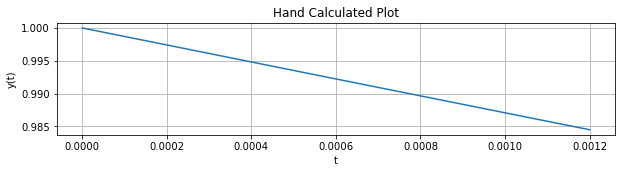
\includegraphics[scale = 0.50]
{txt/Lab6Fig1.png}

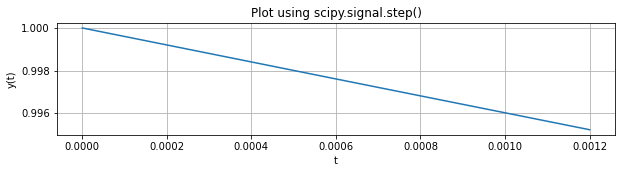
\includegraphics[scale = 0.50]
{txt/Lab6Fig1.5.png}

Figure 2:

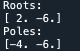
\includegraphics[scale = 0.75]
{txt/Lab6Fig2.png}

Figure 3: 

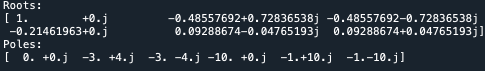
\includegraphics[scale = 0.75]
{txt/Lab6Fig3.png}

Figure 4:

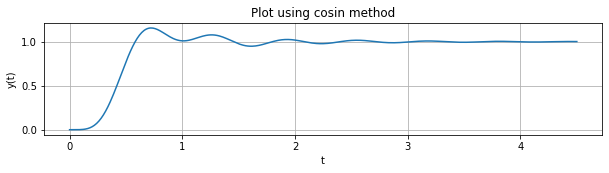
\includegraphics[scale = 0.5]
{txt/Lab6Fig4.png}

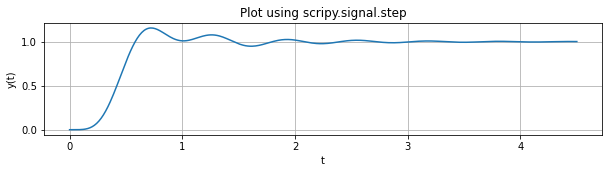
\includegraphics[scale = 0.5]
{txt/Lab6Fig4.5.png}

\begin{center}
    Conclusion
\end{center}
    This lab helped me gain a better understanding of the tools that I can use in python to help solve differential equations. The signal command can take a transfer function and plot it as if it was in the time domain. The residue() function can be used to solve roots and poles of our transfer function. These found parameters can tel use alot about our differentail equaiton.
\end{document}

%%%%%%%%%%%%%%%%%%%%%%%%%%%%%%%%%%%%%%%%

% Copyright Remarks:
%--------------------

% Copyright holder: Vebjørn S. Førde, copyright: CC BY 4.0
% Note: The author of this template is also the copyright holder.

% Below is an explanation of the CC BY 4.0. Additional statements/ 
% clarifications made by the author/copyright holder are marked with *.

% YOU ARE FREE TO:
% Share — copy and redistribute the material in any medium or format
% Adapt — remix, transform, and build upon the material
% for any purpose, even commercially.

% UNDER THE FOLLOWING TERMS:
% Attribution* — You must give appropriate credit, provide a link to the license,
% and indicate if changes were made. You may do so in any reasonable manner, but 
% not in any way that suggests the licensor endorses you or your use.

% *Note: 
% Attribution NOT NEEDED for: 
%       - PDF distibution (like sharing your PDF document)
%       - Use of (dummy)text and images provided in the template (obviously)
%       - Distributing parts of the template, and not the template as a whole
% I am not really concerned with being given credit. As long as you do not 
% claim to have made the template yourself in distributing it further, I have
% no complaints.

% No additional restrictions — You may not apply legal terms or technological 
% measures that legally restrict others from doing anything the license permits.

% NOTICES:
% No warranties are given.

% Disclaimer* (added by copyright holder):
% THE SOFTWARE IS PROVIDED "AS IS", WITHOUT WARRANTY OF ANY KIND, EXPRESS OR
% IMPLIED, INCLUDING BUT NOT LIMITED TO THE WARRANTIES OF MERCHANTABILITY,
% FITNESS FOR A PARTICULAR PURPOSE AND NONINFRINGEMENT. IN NO EVENT SHALL THE
% AUTHORS OR COPYRIGHT HOLDERS BE LIABLE FOR ANY CLAIM, DAMAGES OR OTHER
% LIABILITY, WHETHER IN AN ACTION OF CONTRACT, TORT OR OTHERWISE, ARISING FROM,
% OUT OF OR IN CONNECTION WITH THE SOFTWARE OR THE USE OR OTHER DEALINGS IN THE
% SOFTWARE.

% Read more about CC BY 4.0:
% https://creativecommons.org/licenses/by/4.0/